% !TEX program = xelatex
\documentclass[12pt,a4paper]{article}

%%
% CUMCM 数学建模竞赛论文写作培训模板（2026规范+AI规定内嵌版）
% 用法：本文件既可作为培训讲义，也可作为参赛论文写作母版。
% 正式参赛时：删除所有“【培训提示】”文字、示例性内容，并替换为本队实际内容。
%%

\usepackage{geometry}
\geometry{a4paper,left=2.5cm,right=2.5cm,top=2.5cm,bottom=2.5cm}
\usepackage{ctex}
\usepackage{sectsty}
\sectionfont{\centering}
\renewcommand\thesection{\chinese{section}、}
\renewcommand\thesubsection{\arabic{section}.\arabic{subsection}}
\usepackage[dvipsnames]{xcolor}
\usepackage{booktabs}
\usepackage{makecell}
\usepackage{amsfonts,amsmath,amssymb,mathtools}
\usepackage{multirow}
\usepackage{graphicx}
\usepackage{subcaption}
\usepackage{float}
\usepackage{enumitem}
\usepackage{array}
\usepackage{longtable}
\usepackage{listings}
\usepackage{fancyhdr}
\usepackage{hyperref}
\usepackage{url}

\hypersetup{
  colorlinks=true,
  linkcolor=black,
  urlcolor=blue,
  citecolor=black,
  pdfstartview=Fit,
  breaklinks=true
}

\lstset{
  frame=tb,
  aboveskip=3mm,
  belowskip=3mm,
  showstringspaces=false,
  columns=flexible,
  framerule=1pt,
  rulecolor=\color{gray!35},
  backgroundcolor=\color{gray!5},
  basicstyle={\small\ttfamily},
  numbers=left,
  numberstyle=\tiny\color{gray},
  keywordstyle=\color{blue},
  commentstyle=\color{ForestGreen},
  breaklines=true,
  breakatwhitespace=true,
  tabsize=3
}
\renewcommand{\lstlistingname}{源程序}

\newcommand{\tip}[1]{\par\noindent\textbf{【提示】} #1\par}
\newcommand{\warning}[1]{\par\noindent\textbf{【高频失分点】} #1\par}
\newcommand{\good}[1]{\par\noindent\textbf{【推荐写法】} #1\par}
\newcommand{\bad}[1]{\par\noindent\textbf{【不推荐写法】} #1\par}
\newcommand{\core}[1]{\boxed{\text{#1}}}

\fancyhf{}
\cfoot{\thepage}
\renewcommand{\headrulewidth}{0pt}
\pagestyle{fancy}

\begin{document}

% ============================================================
% 摘要页：电子版第一页，页码从1开始
% ============================================================
\pagenumbering{arabic}
\setcounter{page}{1}

\begin{center}
{\zihao{-2}\bfseries 论文标题（在原题目上加上亮点或主要工作）}

\vspace{2ex}
{\zihao{3}\bfseries 摘要}
\end{center}

本文针对XXX问题，建立XXX模型与XXX模型，研究XXX与XXX之间的关系。首先，根据题目给出的XXX条件，作出XXX假设，将实际问题中的XXX量化为XXX变量，建立XXX模型；其次，采用XXX方法求解模型，并针对XXX困难设计/改进XXX算法；最后，通过XXX数据、XXX指标和XXX检验对模型进行验证，得到XXX结论。

针对问题1，建立XXX模型，采用XXX方法求解，得到XXX主要结果；针对问题2，在问题1模型的基础上进一步考虑XXX因素，建立XXX模型，得到XXX结果；针对问题3，综合XXX与XXX，建立XXX优化模型，提出XXX策略。结果表明，XXX参数变化将导致XXX变化，最优方案为XXX，相关指标达到XXX。

模型的优点在于XXX；通过灵敏度分析/误差分析发现XXX；在放宽XXX假设后，模型仍具有XXX应用潜力。

\vspace{2ex}
\noindent{\heiti 关键词：} 数学建模；XXX模型；XXX算法；XXX优化；灵敏度分析

\vspace{2ex}
\tip{摘要专用页原则上不超过一页；摘要、正文、附录中任何地方都不能出现参赛者身份、所在学校及赛区信息；页码从摘要页开始，以阿拉伯数字1连续编号，位于页脚中部。不写英文摘要。摘要不是“目录式介绍”，而是一页内让评阅人回答四个问题：\textbf{研究什么、怎么建模、怎么求解、得到什么结论}。  

一个好摘要至少应出现若干“可核验”的结果，例如“预测误差降低至X\%”“最优方案使成本下降X\%”“温度峰值达到X℃”“准确率为X\%”。如果全文最有价值的结论没有进入摘要，评阅人很容易错过论文亮点。}

\begin{table}[H]
\centering
\caption{摘要逐句检查表}
\begin{tabular}{p{2.8cm}p{10.5cm}}
\toprule
句子功能 & 应回答的问题 \\
\midrule
背景与目标 & 现实问题是什么？本文究竟解决什么？ \\
模型概述 & 建立了什么模型？核心变量和关系是什么？ \\
求解方法 & 用什么算法/理论方法？为什么适合？ \\
主要结果 & 最重要的数值、排序、趋势或最优方案是什么？ \\
结论与应用 & 结果说明什么？能用于什么决策？ \\
\bottomrule
\end{tabular}
\end{table}

\warning{摘要中避免“本文首先$\cdots$其次$\cdots$最后$\cdots$”连续堆砌过程，却不明确写出算出了什么；避免“结果很好、模型合理、效果显著”等没有数据支撑的空泛表述。}

 

\clearpage

% ============================================================
% 一、问题重述
% ============================================================
\section{问题重述}

\tip{问题重述的任务不是“复印题目”，而是把题目翻译成数学建模语言。建议压缩原题背景，保留真正影响模型的条件、目标和输出。}

\subsection{问题背景}

用自己的语言概括现实背景。若背景涉及成熟理论、公开数据或他人研究，可引用1--3篇高质量文献，并用一句话说明文献与本文的关系。\

\good{“已有研究表明，XX变化会显著影响产品质量。针对XX的约束与目标温度，本文进一步考虑XX，建立XX优化模型。”}
\bad{“某某是非常重要的问题，在现实生活中有广泛应用，因此我们研究它。”}

\subsection{问题重述}

建议将每个子问题压缩为一段，统一采用：
\[
\text{已知条件}\rightarrow\text{决策变量}\rightarrow\text{模型任务}\rightarrow\text{输出结果}
\]

\begin{table}[H]
\centering
\caption{问题重述的四要素}
\begin{tabular}{p{3cm}p{10cm}}
\toprule
要素 & 写作内容 \\
\midrule
已知条件 & 数据、边界、物理规律、题目给定约束 \\
决策变量 & 哪些量可以控制、优化或预测 \\
模型任务 & 拟合、预测、分类、评价、优化、调度、仿真等 \\
输出结果 & 数值、排序、最优方案、策略、敏感因素等 \\
\bottomrule
\end{tabular}
\end{table}

\warning{绝对避免大段照抄题面。即使没有查重要求，照抄也会浪费正文篇幅，并且无法体现建模能力。}

% ============================================================
% 二、问题分析
% ============================================================
\section{问题分析}

这一部分体现“从实际问题到数学问题”的思维过程。核心不是介绍算法，而是解释\textbf{为什么这样建模}。

\[
\boxed{\text{题目给了什么？}\quad\text{真正难点是什么？}\quad\text{准备怎样把它数学化？}}
\]

\tip{问题分析通常控制在每个问题4--10行，但信息密度要高。不要在这里提前公布详细计算结果；模型公式放到后面的“模型建立”。}

\subsection{问题1的分析}

从数据结构、变量关系、约束条件、目标函数、模型难点五个角度分析。尤其指出哪些信息可以直接利用，哪些信息需要作假设或转换。

\good{“问题1的核心是根据离散测量数据确定控制变量与温度之间的映射关系。由于温度曲线具有明显的时序特征，直接采用静态回归会忽略相邻时刻的相关性，因此先对数据进行平滑处理，再建立动态模型，并以题目给出的温度上限、变化速率和终点要求作为约束。”}

\subsection{问题2的分析}

强调模型继承关系：
\[
M_1\quad\longrightarrow\quad M_1+\text{新条件}\quad\longrightarrow\quad M_2.
\]

\tip{“问题2在问题1基础上增加一个因素”本身不是分析。要说明新增因素进入哪个变量、改变哪条约束、是否改变目标函数，以及为什么原算法需要调整。}

\subsection{问题3的分析}

复杂问题可拆解为：
\[
\text{数据处理}\rightarrow\text{基础模型}\rightarrow\text{预测/评价}\rightarrow\text{优化}\rightarrow\text{方案比较}. 
\]

\tip{如果一个问题同时出现“预测+优化”，最好把两者的接口写清楚：预测模型输出什么量，优化模型把它作为参数还是约束，最终如何形成决策。}

% ============================================================
% 三、模型假设
% ============================================================
\section{模型假设}

\tip{好的假设不是越多越好，而是“必要、合理、可解释、能降低复杂度”。每一个关键假设最好能回答：为什么需要？违反它会怎样？是否会影响结论？} 常见假设来源：
\begin{enumerate}[label=(\arabic*)]
  \item 题目明确给出的条件；
  \item 排除极低概率或明显异常事件；
  \item 忽略对目标影响很小的次要因素；
  \item 某经典模型或算法所要求的技术假设；
  \item 对未知参数、分布、噪声形式作合理假设；
  \item 为使模型可计算而进行的合理离散化或近似。
\end{enumerate}

\begin{table}[H]
\centering
\caption{模型假设的推荐写法}
\begin{tabular}{p{2cm}p{5cm}p{6cm}}
\toprule
假设类型 & 不推荐 & 推荐 \\
\midrule
数据异常 & 数据没有问题 & 剔除明显录入错误及超出物理范围的异常点，并保留处理规则 \\
次要因素 & 其他因素忽略 & 经量纲/数量级分析，次要因素相对于主导因素影响可忽略 \\
随机性 & 假设数据服从正态分布 & 通过QQ图/检验/领域知识说明采用该分布的依据 \\
简化 & 为了方便计算 & 在不改变主要趋势和核心约束的前提下进行合理简化 \\
\bottomrule
\end{tabular}
\end{table}

\warning{不要把“假设模型结果正确”“假设结果符合预期”写进模型假设。这是循环论证。}

% ============================================================
% 四、符号说明
% ============================================================
\section{符号说明}

\tip{只列核心变量。临时求和指标、简单中间变量不必全部塞进符号表，但正文首次出现时仍应解释。符号应尽量有含义，避免同一个字母在不同章节代表不同变量。}

\begin{table}[H]
\centering
\caption{主要符号说明}
\label{tab:symbol}
\begin{tabular}{p{3cm}p{8cm}p{2cm}}
\toprule
符号 & 说明 & 单位\\
\midrule
$T$ & 系统运行时间 & min\\
$u_i$ & 第 $i$ 个时刻的控制输入 & --\\
$x_i$ & 第 $i$ 个决策变量 & --\\
$y_i$ & 第 $i$ 个观测/响应量 & --\\
$\mathbb{E}[X]$ & 随机变量 $X$ 的数学期望 & --\\
$J$ & 优化目标函数 & --\\
\bottomrule
\end{tabular}
\end{table}

\tip{符号设计的经验：优先使用约定俗成记号；没有约定时可用英文含义前缀，如 $T_{\max}$、$T_{\mathrm{tol}}$、$C_{\mathrm{cost}}$；关键决策变量可直接使用 $x_i$。不要为了“高级”而使用过于复杂的希腊字母。}

% ============================================================
% 五、模型建立与求解
% ============================================================
\section{模型的建立与求解}

\tip{这是全文核心。评阅人真正关心的是：从题目条件怎样得到数学关系？模型是否闭合？变量、参数、约束、目标是否定义清楚？算法能否真正求出这个模型？}

\subsection{建模总路线：从文字到公式}

\[
\boxed{
\text{题目条件}
\rightarrow
\text{变量定义}
\rightarrow
\text{基本规律}
\rightarrow
\text{数学关系}
\rightarrow
\text{约束}
\rightarrow
\text{目标函数}
\rightarrow
\text{完整模型}
}
\]

\begin{table}[H]
\centering
\caption{不同题型的核心模型结构}
\begin{tabular}{p{3cm}p{11cm}}
\toprule
题型 & 论文中必须交代的核心内容 \\
\midrule
预测 & 数据预处理、特征、模型、训练/拟合、误差指标、预测结果 \\
评价 & 指标体系、权重、标准化、综合评价、稳健性检验 \\
优化 & 决策变量、目标函数、约束、求解算法、最优方案 \\
分类 & 特征、标签、训练策略、评价指标、分类结果 \\
聚类 & 距离/相似度、类别数、聚类算法、稳定性、类别解释 \\
微分方程 & 状态变量、机理方程、初边值条件、参数、数值方法 \\
图论/网络 & 节点、边、权重、路径/流/连通性定义及算法 \\
\bottomrule
\end{tabular}
\end{table}

\subsection{问题1模型的建立与求解}

\subsubsection{模型的建立}

模型可以来自经典模型，但不能“见到关键词就套模型”。应明确说明题目信息如何映射到模型参数与结构。

\paragraph{例1：一般优化模型}
\begin{equation}
\begin{aligned}
\max_{x}\quad & f(x)\\
\text{s.t.}\quad & g_i(x)\le 0,\quad i=1,\ldots,m,\\
& h_j(x)=0,\quad j=1,\ldots,p,\\
& x\in\mathcal X.
\end{aligned}
\end{equation}

\paragraph{例2：微分方程}
\begin{equation}
\left\{
\begin{aligned}
\dot{x}(t)&=f(x(t),u(t),t),\\
 y(t)&=g(x(t),u(t),t),\\
 x(0)&=x_0.
\end{aligned}
\right.
\end{equation}

\paragraph{例3：线性规划/整数规划}
\begin{equation}
\begin{aligned}
\min\quad & c^{\mathsf T}x\\
\text{s.t.}\quad & Ax\le b,\\
& x\ge0,\qquad x_i\in\mathbb Z\ \text{(若需要)}.
\end{aligned}
\end{equation}

\tip{模型公式出现后，必须“翻译”公式：目标函数代表什么？每条约束对应题目的哪句话？变量取值范围为什么这样设？这一步往往比写公式本身更能体现建模能力。}

\subsubsection{模型的求解}

算法描述不宜写成教材。只写与本题有关的核心步骤。

\begin{description}
\item[第1步：] 数据预处理、缺失值处理、异常值处理、标准化或参数初始化；
\item[第2步：] 根据模型结构生成参数、约束和初始解；
\item[第3步：] 使用XXX方法求解，并设置合理的终止准则；
\item[第4步：] 对候选解进行可行性检查；
\item[第5步：] 输出最优解/预测值/分类结果，并进行独立验证。
\end{description}

\tip{写算法时优先回答“为什么选它”，其次才是“怎么跑”。例如：整数规划适用于离散决策且约束线性；遗传算法适合非凸、非线性、组合优化但需要说明编码、适应度、交叉、变异和终止准则；神经网络必须说明输入输出、训练数据、损失函数及验证方式。}

\subsection{问题2模型的建立与求解}

\tip{问题2最容易写成“重复问题1”。建议显式指出：问题1的哪些变量、参数、结论被继承？新增条件改变了什么？因此模型发生了什么变化？}

\[
M_1=(F_1,\mathcal C_1)\quad\longrightarrow\quad
M_2=(F_2,\mathcal C_1\cup\mathcal C_{\mathrm{new}}).
\]

\subsection{问题3模型的建立与求解}

复杂问题可以采用模块化结构：
\[
M_3=M_{\mathrm{data}}+M_{\mathrm{predict}}+M_{\mathrm{evaluate}}+M_{\mathrm{opt}}.
\]

\tip{如果使用“预测+优化”的组合模型，要写清楚误差如何传递。例如预测模型输出 $\hat y$，优化模型以 $\hat y$ 为输入；进一步可通过情景分析或鲁棒优化检验预测误差对最终方案的影响。}

% ============================================================
% 六、数据处理与统计建模干货
% ============================================================
\section{数据处理：最容易被忽视，却最容易出问题}

\subsection{数据预处理的基本原则}

完整流程建议：
\[
\text{原始数据}
\rightarrow\text{格式检查}
\rightarrow\text{缺失值}
\rightarrow\text{异常值}
\rightarrow\text{重复值}
\rightarrow\text{单位统一}
\rightarrow\text{标准化}
\rightarrow\text{建模数据}.
\]

\begin{table}[H]
\centering
\caption{常见数据问题及处理方法}
\begin{tabular}{p{1.8cm}p{6cm}p{7cm}}
\toprule
问题 & 常用方法 & 注意事项 \\
\midrule
缺失值 & 删除、均值/中位数、插值 & 不能无理由删除关键样本 \\
异常值 & 箱线图、3$\sigma$、IQR、稳健方法 & 先判断是错误还是有意义的极端事件 \\
量纲不同 & Min-Max、Z-score等 & 权重评价、聚类、距离模型尤其敏感 \\
时间序列 & 插值、平滑、滞后变量 & 不要随机打乱时间序列训练/测试集 \\
类别变量 & 独热编码、序数编码 & 编码方式必须符合变量含义 \\
\bottomrule
\end{tabular}
\end{table}

\warning{“删除异常值后模型效果更好”不能作为删除理由。必须先从题目背景或数据生成机制解释异常值是否属于错误数据。}

\subsection{统计模型不要只报一个 $R^2$}

回归类问题至少考虑：
\[
\mathrm{MAE}=\frac1n\sum_{i=1}^n|y_i-\hat y_i|,
\qquad
\mathrm{RMSE}=\sqrt{\frac1n\sum_{i=1}^n(y_i-\hat y_i)^2},
\qquad
R^2=1-\frac{\sum_i(y_i-\hat y_i)^2}{\sum_i(y_i-\bar y)^2}.
\]

\tip{$R^2$高并不自动意味着预测好。尤其在外推问题、异常点明显、样本很少时，应增加留出验证、交叉验证、残差图或实际数据检验。}

% ============================================================
% 七、算法写作
% ============================================================
\section{算法写作：不要把论文写成算法说明书}

\subsection{算法选择的“理由链”}

\[
\boxed{\text{模型性质}\rightarrow\text{算法性质}\rightarrow\text{选择理由}\rightarrow\text{改进点}\rightarrow\text{验证}}
\]

\begin{table}[H]
\centering
\caption{常见算法与论文写作重点}
\begin{tabular}{p{4cm}p{12cm}}
\toprule
方法 & 论文重点 \\
\midrule
线性/整数规划 & 变量、目标、约束、整数性；求解器及最优性/可行性检查 \\
遗传算法 & 编码、适应度、选择、交叉、变异、终止条件、重复运行稳定性 \\
粒子群算法 & 粒子表示、速度位置更新、参数、终止准则、随机性处理 \\
模拟退火 & 邻域、能量函数、降温策略、接受准则 \\
神经网络 & 输入输出、网络结构、损失函数、训练/验证划分、过拟合控制 \\
随机森林/XGBoost & 特征、训练策略、评价指标、特征重要性、泛化检验 \\
聚类 & 距离、类别数选择、聚类质量指标、结果解释 \\
\bottomrule
\end{tabular}
\end{table}

\warning{“采用遗传算法求解，得到结果如下”通常信息量太低。评阅人不知道你为什么用它、怎样编码、结果是否稳定。}

\tip{智能优化算法的结果具有随机性时，建议重复运行多次，报告最优值、均值、标准差或稳定区间；如果只给一次运行结果，难以判断算法偶然性。}

% ============================================================
% 八、结果展示
% ============================================================
\section{结果展示：图、表、公式必须服务于结论}

\tip{图表不是“有图就加分”。高质量图表应该让评阅人在几秒内找到趋势、差异、最优方案或异常点。}

\begin{figure}[htb]
    \centering
    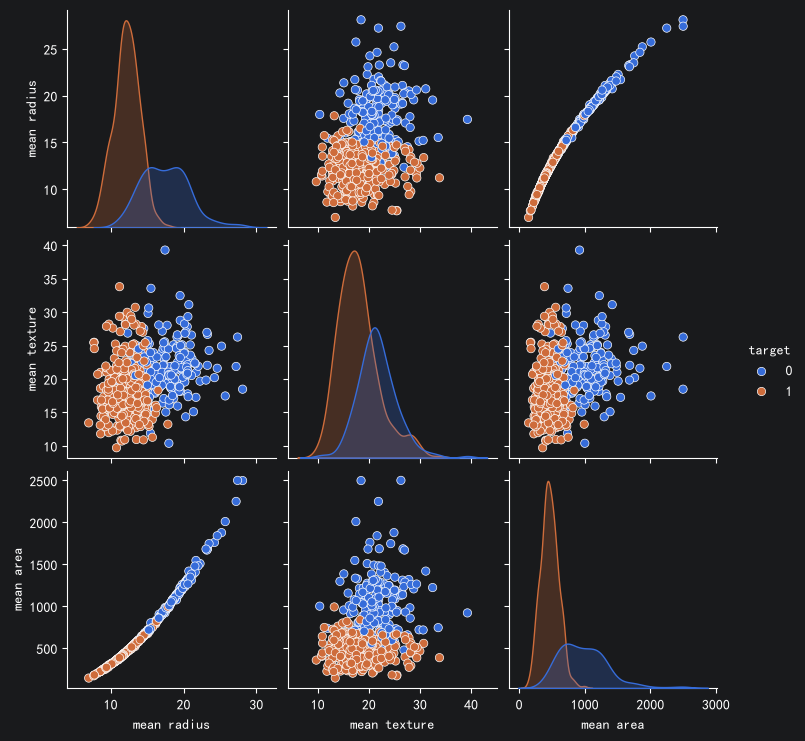
\includegraphics[width=0.85\linewidth]{figure1.png}
    \caption{特征配对分布图}
    \label{fig:placeholder}
\end{figure}



\begin{table}[H]
\centering
\caption{结果展示示例}
\label{tab:result}
\begin{tabular}{ccccc}
\toprule
方案 & 指标1 & 指标2 & 综合指标 & 排名\\
\midrule
A & 10.2 & 5.1 & 0.82 & 2\\
B & 12.5 & 4.7 & 0.91 & 1\\
C & 11.1 & 6.2 & 0.78 & 3\\
\bottomrule
\end{tabular}
\end{table}

图表之后建议采用：
\[
\boxed{\text{现象}\rightarrow\text{定量比较}\rightarrow\text{原因解释}\rightarrow\text{结论}}
\]

\good{“由表\ref{tab:result}可见，方案B的综合指标为0.91，在三种方案中最高；相较方案A提高约11.0\%，说明在当前权重设置下，增加XXX因素能够显著改善综合表现。因此后续将方案B作为基准方案进行灵敏度分析。”}

\bad{“由表可知，B最好，说明模型很好。”}

\subsection{图表规范}
\begin{itemize}
  \item 图、表必须有编号和标题；
  \item 表格优先使用三线表，非必要不使用竖线；
  \item 图中坐标轴必须写清变量名和单位；
  \item 图例、字号、线宽应保证打印后清晰；
  \item 图表中的数据应与正文完全一致；
  \item 正文必须解释关键图表，不能“甩图”；
  \item label 放在 caption 后面，便于交叉引用；
  \item 不要用截图代替可编辑的高质量图形。
\end{itemize}

\subsection{推荐图形清单}
\begin{table}[H]
\centering
\caption{不同目的的推荐图形}
\begin{tabular}{p{4cm}p{8.5cm}}
\toprule
目的 & 推荐图形 \\
\midrule
趋势变化 & 折线图、时间序列图 \\
变量关系 & 散点图、拟合曲线、相关矩阵 \\
误差分析 & 残差图、误差分布图、箱线图 \\
方案比较 & 柱状图、雷达图（慎用）、平行坐标图 \\
空间问题 & 热力图、等值线图、散点地图 \\
网络问题 & 网络图、最短路可视化、流量图 \\
算法稳定性 & 收敛曲线、箱线图、重复实验统计 \\
\bottomrule
\end{tabular}
\end{table}

% ============================================================
% 九、模型检验、误差、灵敏度、稳健性
% ============================================================
\section{模型检验、误差分析、灵敏度与稳健性}

\subsection{模型检验}

至少选择一种与问题性质匹配的验证方式：
\begin{itemize}
  \item 已知数据回代验证；
  \item 留出集/交叉验证；
  \item 与经典模型或基准方案比较；
  \item 极端情形测试；
  \item 真实案例验证；
  \item 约束可行性与物理意义检查。
\end{itemize}

\tip{优化题不要只验证“目标函数更大/更小”，还要检查约束是否全部满足；预测题不要只展示拟合曲线，还要检查预测误差；评价题要检查权重变化是否导致排名剧烈翻转。}

\subsection{误差分析}

可从三类误差讨论：
\[
\text{数据误差}+\text{模型误差}+\text{数值计算误差}.
\]

\begin{itemize}
  \item 数据误差：测量误差、缺失、噪声、抽样偏差；
  \item 模型误差：简化假设、变量遗漏、结构偏差；
  \item 数值误差：离散化、迭代终止、浮点误差、算法近似。
\end{itemize}

\subsection{灵敏度分析}

固定其他参数，仅改变关键参数 $p$：
\[
p\in\{0.8p_0,0.9p_0,p_0,1.1p_0,1.2p_0\},
\]
观察结果 $Y(p)$ 的变化。更严格时可以报告局部敏感度：
\[
S_p=\frac{p}{Y}\frac{\partial Y}{\partial p}.
\]

\tip{灵敏度分析不是“多跑几次程序”。必须说明为什么选择这个参数、变化范围为什么合理，以及结果变化是否会改变最终决策。}

\subsection{稳健性分析}

如果模型用于决策，建议增加：
\[
\text{参数扰动}\rightarrow\text{重新求解}\rightarrow\text{方案排名/最优解}\rightarrow\text{稳定性结论}.
\]

\tip{“最优值变化很小”只是数值结论；更有价值的是“在合理参数区间内，最优方案始终为B，因此决策具有稳健性”。}

% ============================================================
% 十、模型评价与推广
% ============================================================
\section{模型的评价与推广}

\subsection{模型的优点}

建议从以下角度选择2--4点：
\begin{enumerate}
  \item 针对性：准确对应题目关键条件；
  \item 可解释性：参数和结果具有明确实际含义；
  \item 计算效率：在保证精度的前提下减少计算量；
  \item 稳定性：参数扰动下结果保持稳定；
  \item 泛化性：可以迁移到类似场景；
  \item 创新性：改进模型结构、目标函数或求解算法。
\end{enumerate}

\subsection{模型的缺点}

真实说明模型边界，例如：
\begin{itemize}
  \item 由于数据样本有限，无法进一步刻画XXX因素；
  \item 为降低模型复杂度，将XXX过程近似为XXX；
  \item 智能优化算法存在随机性，仍需更多重复实验验证；
  \item 某些参数依赖公开资料，可能存在地区或时间差异。
\end{itemize}

\warning{缺点不是“为了谦虚而写”，而是要和模型假设、误差分析呼应。优点数量通常可以多于缺点，但不要声称模型“完美、完全准确、适用于所有情况”。}

\subsection{模型推广}

推广最好形成“放宽一个假设”的具体路线：
\[
\text{当前模型}
\rightarrow\text{放宽假设}
\rightarrow\text{增加变量/约束}
\rightarrow\text{升级算法}
\rightarrow\text{实际应用}.
\]

\good{“若进一步考虑需求具有随机波动的情形，可将确定性参数替换为随机变量，并在现有优化模型基础上构造机会约束模型；若要求在最坏情况下仍保持可行，则可进一步研究鲁棒优化模型。”}

% ============================================================
% 十一、创新与亮点
% ============================================================
\section{如何制造真正的“亮点”，而不是堆算法}

\tip{数学建模竞赛的创新通常不是“用了一个听起来很新的算法”，而是把题目中的特殊条件转化成模型结构、指标设计或求解策略。}

\begin{table}[H]
\centering
\caption{常见有效亮点}
\begin{tabular}{p{3.5cm}p{9cm}}
\toprule
亮点层次 & 具体表现 \\
\midrule
问题转化 & 把模糊实际描述转成清晰变量、指标和约束 \\
模型结构 & 在经典模型基础上增加题目特有机制 \\
指标设计 & 构造更符合实际目标的评价指标/综合目标 \\
算法改进 & 针对本题瓶颈修改初始化、搜索、约束处理等 \\
模型融合 & 预测、评价、优化之间形成闭环 \\
稳健性 & 对参数、噪声、数据变化进行系统检验 \\
可解释性 & 能回答“为什么得到这个结果”而不只是给数值 \\
\bottomrule
\end{tabular}
\end{table}

\warning{“使用遗传算法+BP神经网络+灰色预测+TOPSIS”不等于创新。算法越多，越要说明每一个模块解决什么具体问题，否则容易变成“算法大杂烩”。}

\subsection{一个很实用的创新公式}
\[
\boxed{\text{题目特殊条件}+\text{经典模型缺陷}+\text{针对性改进}=\text{可信亮点}}
\]

% ============================================================
% 十二、参考文献
% ============================================================
\section{参考文献}

\tip{所有引用他人或公开资料（包括网上资料）的成果都必须按科技论文规范列出参考文献，并在正文引用处标注。不要为了“凑文献”而引用与本文无关的论文。}

\begin{enumerate}
  \item 优先使用原始论文、官方报告、权威数据库和教材；
  \item 引用文献必须能在正文中找到对应位置；
  \item 网上资料应尽可能记录标题、机构、发布日期/访问日期等信息；
  \item 不要直接复制二手资料的参考文献表；
  \item 论文中的数字、公式、方法来源若来自他人工作，应明确引用。
\end{enumerate}

\tip{参考文献的真正作用是告诉评阅人：哪些是已有知识，哪些是你们队自己的工作。越是核心模型、关键数据和特殊算法，越要注意知识来源边界。}

% ============================================================
% 十三、AI工具使用声明——嵌入正文，不另放外部说明
% ============================================================
\section*{AI工具使用声明}

\tip{以下规定按照题目所提供的《全国大学生数学建模竞赛人工智能工具使用规定（2026年试行）》整合进模板。该规定自2026年9月1日起试行。正式比赛必须依据实际使用情况二选一，不能两段同时保留。}

\subsection*{2026年AI工具使用规定要点}
\begin{enumerate}
  \item AI工具包括但不限于大语言模型、生成式AI、代码辅助工具和AI智能体；
  \item 竞赛不要求必须使用AI；参赛队可以使用，但必须遵循公开透明原则；
  \item \textbf{核心建模与分析必须由参赛队主导}；
  \item 对AI参与完成的内容必须逐项进行人工审查与核实；
  \item 使用AI的参赛作品，须在参考文献之前设置AI工具使用声明；
  \item 使用AI的参赛作品，还须在支撑材料中提供PDF文件“\texttt{AI工具使用详情.pdf}”；
  \item AI详情至少说明：工具名称及版本/型号、使用目的和环节、主要提示方式与过程、AI输出的采纳/修改/核验情况；
  \item 故意隐瞒AI使用、作出虚假声明，或把未经必要人工审查与核实的AI生成内容直接作为核心建模与分析成果提交，可能被取消评奖资格。
\end{enumerate}

\subsection*{方案A：未使用AI工具}
\begin{quote}
\textbf{本参赛队在竞赛过程中未使用任何AI工具。}
\end{quote}

\subsection*{方案B：使用AI工具}
\begin{quote}
\textbf{本参赛队在竞赛过程中使用了AI工具，主要用于【简要用途，如语言润色、代码调试等】，详细使用情况见支撑材料。}
\end{quote}

\warning{正式论文必须二选一，并且必须与实际情况一致。不能为了“看起来规范”而选择“未使用AI”，也不能把实际发生的AI使用范围写得过于模糊。}

\subsection*{AI使用的边界：什么可以做，什么必须自己做？}

\begin{table}[H]
\centering
\caption{AI辅助数学建模的风险分级建议}
\begin{tabular}{p{3.5cm}p{1cm}p{7.5cm}}
\toprule
环节 & 风险 & 建议 \\
\midrule
语言润色、错别字 & 较低 & 人工通读，确认没有改变数学含义 \\
代码语法调试 & 中低 & 必须自己运行并检查输出 \\
公式排版、LaTeX & 中低 & 编译并逐式核对 \\
算法思路建议 & 中 & 必须理解并独立验证适用条件 \\
数据处理方案 & 中高 & 核查数据来源、处理规则和统计合理性 \\
核心模型推导 & 高 & 逐步验证，不能直接照搬AI答案 \\
最终结论 & 高 & 必须由实际计算/实验结果支撑 \\
\bottomrule
\end{tabular}
\end{table}

\tip{一个非常实用的原则：\textbf{“AI可以建议，不能替你负责。”}任何进入最终论文的公式、代码、数字、算法、结论，都应该能够由队员解释、复现和核验。}

% ============================================================
% 十四、附录与支撑材料
% ============================================================
\clearpage
\appendix
\section{支撑材料列表}

\tip{2026年修订稿：附录页数不限，附录内容必须打印并与正文装订。支撑材料应包含用于支撑模型、结果、结论的必要材料，至少包括完整可运行源程序、自主查阅使用的数据资料（赛题原始数据除外）、较大篇幅中间结果图表等。}

\begin{enumerate}
  \item \texttt{problem1\_main.m}：问题1完整程序；
  \item \texttt{problem2\_main.m}：问题2完整程序；
  \item \texttt{data\_source.xlsx}：自主查阅数据；
  \item \texttt{intermediate\_results.xlsx}：较大篇幅中间结果；
  \item \texttt{AI工具使用详情.pdf}：若使用AI，必须提供；
  \item 其他能够复现实验、图表和关键结论的必要文件。
\end{enumerate}

\warning{支撑材料不是“把代码随便打包”。程序必须完整、可运行，且运行结果与论文一致；文件之间应有清晰的命名和目录结构。}

\section{AI工具使用详情说明}

\tip{仅当使用AI工具时制作本节对应的独立PDF：\texttt{AI工具使用详情.pdf}。以下内容可以直接作为该PDF的目录和写作框架。}

\subsection*{1. 所用AI工具名称、版本或型号}
\begin{table}[H]
\centering
\caption{AI工具信息记录模板}
\begin{tabular}{p{2cm}p{2cm}p{7cm}}
\toprule
工具名称 & 版本/型号 & 使用环节 \\
\midrule
XXX & XXX & 语言润色/代码调试/方案讨论 \\
XXX & XXX & XXX \\
\bottomrule
\end{tabular}
\end{table}

\subsection*{2. 具体使用目的和环节}
建议按照“时间/环节—目的—输出—人工处理”记录。

\begin{table}[H]
\centering
\caption{AI使用过程记录模板}
\begin{tabular}{p{2.2cm}p{3.5cm}p{3cm}p{5cm}}
\toprule
环节 & 使用目的 & AI输出内容 & 人工处理 \\
\midrule
建模前 & 文献/思路整理 & XXX & 核查文献与适用条件 \\
建模中 & 代码调试 & XXX & 自行运行并修改 \\
写作中 & 语言润色 & XXX & 人工确认数学含义 \\
\bottomrule
\end{tabular}
\end{table}

\subsection*{3. 主要提示方式与使用过程}
可记录典型交互：
\[
\text{任务描述}\rightarrow\text{提示词}\rightarrow\text{AI建议}\rightarrow\text{人工筛选}\rightarrow\text{实际验证}.
\]

\subsection*{4. AI输出的采纳、修改与核验}
至少说明：
\begin{itemize}
  \item 哪些建议被采纳；
  \item 哪些建议被修改；
  \item 哪些建议被舍弃及原因；
  \item 数学推导如何核验；
  \item 代码如何运行核验；
  \item 数据如何交叉核验；
  \item 最终结论如何由独立计算得到。
\end{itemize}

\tip{培训阶段建议比赛全程保留AI使用日志，包括工具名称、日期、关键提示词、重要输出、最终是否采用。这样比赛结束后制作AI详情PDF会非常省力。}

% ============================================================
% 十五、源程序
% ============================================================
\section{源程序}

\tip{2026年修订稿明确要求：建模所用到的全部完整、可运行源程序代码（含EXCEL、SPSS等软件的交互命令）应纳入支撑材料。程序不能运行或运行结果与论文不符，都可能影响评奖资格。}

\begin{lstlisting}[language=matlab,caption={MATLAB完整程序示例}]
% 正式比赛时不要使用“略去”“省略代码”等写法。
% 这里仅展示格式；正式提交应替换为真实、完整、可运行程序。

t = [48.7 53.0 61.3 72.0 48.7 52.0 64.0];
w = [2000 3000 1000 500 4000 2000 1000];
n = [8 7 9 6 6 4 8];

% 数据预处理
% 模型建立
% 参数设置
% 求解
% 结果保存
% 独立验证
\end{lstlisting}

\begin{center}
\textbf{如果确实没有使用任何程序，应在论文附录中明确写：\quad“本论文没有用到程序。”}
\end{center}

% ============================================================
% 十六、2026论文格式规范：完整内嵌版
% ============================================================
% \section{2026年竞赛论文格式规范——提交前必须逐项核对}

% \tip{以下内容根据题目提供的《全国大学生数学建模竞赛论文格式规范（2026年修订稿）》整理，并直接嵌入培训模板。正式参赛前仍应以竞赛组委会发布的最新版本为准。}

% \subsection*{纸质版}
% \begin{enumerate}
%   \item 白色A4纸打印，单面、双面均可；上下左右页边距至少2.5厘米；从左侧装订。
%   \item 第1页为承诺书，第2页为编号专用页。
%   \item 第3页为摘要专用页；摘要含标题和关键词，原则上不超过1页，不需要英文摘要。
%   \item 从摘要页开始编写页码，页码位于页脚中部，以阿拉伯数字1开始连续编号。
%   \item 第4页开始为正文；\textbf{不要目录}；正文不超过30页。
%   \item 正文之后为附录，附录页数不限；附录必须打印并与正文装订提交。
%   \item 摘要、正文和附录任何地方都不能显示参赛者身份、所在学校及赛区信息。
%   \item 所有引用他人或公开资料（包括网上资料）的成果必须按科技论文规范列出参考文献，并在正文引用处标注。
%   \item 未规定的字号、字体、行距、颜色等不统一要求；如赛区另有规定，应同时遵守赛区要求。
% \end{enumerate}

% \subsection*{电子版}
% \begin{enumerate}
%   \item 参赛队提交“参赛论文”和“支撑材料”两个电子文件。
%   \item 参赛论文必须是一个单独文件，PDF或Word二选一，建议PDF；文件大小不超过20MB。
%   \item 电子版论文必须与纸质版内容及格式（包括附录）完全一致。
%   \item \textbf{承诺书和编号专用页不能放入电子版论文}；因此电子版第一页必须是摘要专用页。
%   \item 支撑材料统一压缩为一个RAR或ZIP文件，大小不超过20MB。
%   \item 支撑材料文件列表必须写入论文附录。
%   \item 如果没有支撑材料，可以不提供支撑材料文件，但附录必须注明“本论文没有支撑材料”。
%   \item 承诺书和编号专用页不要放入支撑材料；所有文件中均不得显示参赛者身份、学校及赛区信息。
% \end{enumerate}

% \subsection*{附录与资格风险}
% \begin{itemize}
%   \item 缺少必要源程序；
%   \item 程序无法运行；
%   \item 程序运行结果与论文不一致；
%   \item 支撑材料与论文内容不相符；
%   \item 违反身份信息隐匿要求；
%   \item 不按要求提交AI声明或AI详情材料；
% \end{itemize}
% \textbf{均可能带来严重后果，甚至影响评奖资格。}

% ============================================================
% 十七、最终交稿检查清单
% ============================================================
\section{最终交稿：30分钟“红线检查”}

\begin{longtable}{p{1cm}p{2cm}p{12cm}}
\toprule
序号 & 检查项 & 检查标准 \\
\midrule
1 & 身份信息 & 摘要、正文、附录、支撑材料均无姓名、学校、赛区等身份信息 \\
2 & 页数 & 正文不超过30页；附录不限 \\
3 & 目录 & 正文前没有目录 \\
4 & 页码 & 从摘要页开始为1，页脚中部连续编号 \\
5 & 摘要 & 原则上不超过1页；包含模型、方法、主要结果、结论 \\
6 & 题目重述 & 没有大段复制原题 \\
7 & 模型假设 & 每个关键假设都有实际理由 \\
8 & 符号 & 符号统一、首次出现有解释、单位明确 \\
9 & 模型 & 每个核心问题都有明确数学模型 \\
10 & 约束 & 优化模型的每条关键约束都有现实来源 \\
11 & 算法 & 选择理由、关键步骤、改进点写清楚 \\
12 & 图表 & 编号、标题、单位、图例、数据均正确 \\
13 & 结果 & 正文真正解释了最关键的结果 \\
14 & 检验 & 至少有与问题性质匹配的验证 \\
15 & 灵敏度 & 关键参数变化不会导致结论无故失效，或已说明影响 \\
16 & 评价 & 优缺点与前文假设/检验呼应 \\
17 & 文献 & 每篇引用都在正文出现；每处重要外部资料都有来源 \\
18 & AI声明 & 按实际情况二选一，放在参考文献之前 \\
19 & AI详情 & 使用AI时有“AI工具使用详情.pdf” \\
20 & 源程序 & 全部完整、可运行、结果与论文一致 \\
21 & 支撑材料 & 文件列表写入附录，RAR/ZIP不超过20MB \\
22 & 电子版 & 单独PDF/Word，不含承诺书和编号专用页 \\
23 & 纸质版 & A4、页边距至少2.5cm、左侧装订 \\
24 & 最终复现 & 从零开始运行程序能复现论文关键表格和图形 \\
\bottomrule
\end{longtable}

% ============================================================
% 十八、培训最后强调的“论文高分逻辑”
% ============================================================
\section{培训总结：把论文写成一条完整的证据链}

 

\tip{真正高质量的数模论文不是“公式最多”“算法最复杂”“图最多”，而是每一页都在推进证据链。评阅人能够从题目条件一路追踪到最终结论，并且能够相信：假设合理、模型闭合、算法有效、结果可信、结论可复现。}

\begin{table}[H]
\centering
\caption{一篇优秀数模论文的五个关键词}
\begin{tabular}{p{3cm}p{10cm}}
\toprule
关键词 & 具体含义 \\
\midrule
清楚 & 变量、模型、算法、结果一眼可读 \\
严谨 & 条件、假设、公式、数据、引用均有依据 \\
有效 & 模型真正回答题目，而不是为了套算法 \\
可信 & 有检验、误差、灵敏度或稳健性分析 \\
可复现 & 程序、数据和关键步骤足以复现核心结果 \\
\bottomrule
\end{tabular}
\end{table}

\begin{center}
\vspace{2ex}
\Large\bfseries
不是把“做过的东西”全部写进论文，\par
而是把“最有说服力的证据”组织成一条完整的逻辑链。
\end{center}

\end{document}
